\chapter{Future Work}\label{Sec:Future Work}

Many different adaptations, statistics, and experiments have been left for the future due to lack of time, i.e. data matching and transformation with real data have been very time consuming. Future work concerns deeper analysis of the proposed sampling method, in particular, experiments on synthezised data. Controlled environments are needed to observe the behavior of the proposed algorithm and enable a basis for a more informed exclusion of instances. 

The Synthetic Minority Over-sampling TEchnique (SMOTE [9]) is a very popular oversampling method that creates synthetic minority class instances. The SMOTE instances are linear combinations of two similar instances from the minority class (\(x\) and \(x^{R}\)) and are defined as: \(s = x + u (x^{R} - x) \) with \(0 \geq  u \geq 1\). \(x^{R}\) is randomly chosen among the \(k\) nearest neighbors of \(x\) belonging to the minority class. SMOTE can be used to validate the MRS procedure by simulating the problem at hand.

Specific regions in the feature space are first over-sampled using SMOTE, before they are under-sampled by MRS. Experiments with multiple such synthesized data, with oversampling ratio ranging from high to low, might support the proposed procedure with greater evidence. The initial data sets are then compared to the result sets. GESIS is particularly well suited to artificially recreate the initial problem as visualized in Figure 5.1. It is only necessary to try to avoid giving the synthesized data properties that makes it possible for a learning algorithm to distinguish synthesized from non-synthesized example. This mechanism would for instance aid to compare classification results more easily.

\begin{figure}[ht]
	\begin{center}
\vspace{0.5cm}
		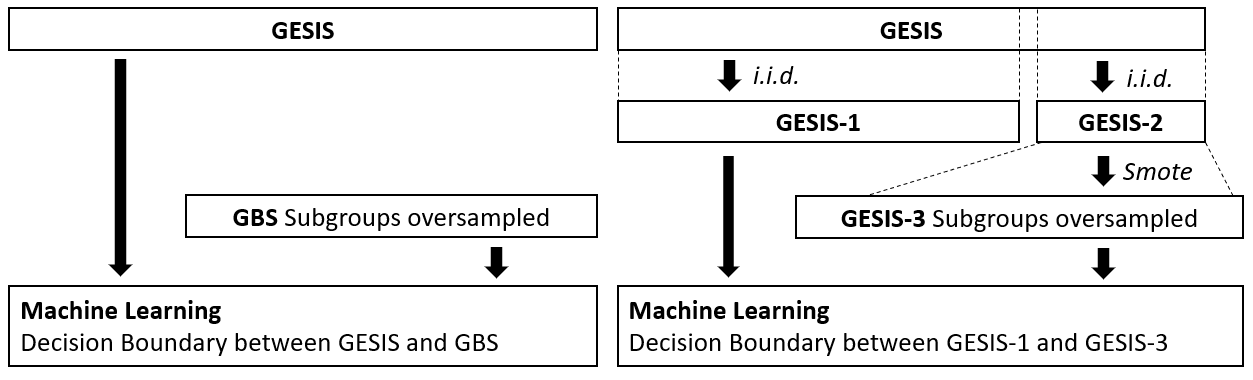
\includegraphics[scale=0.38,angle=0]{fig/procedure2}
		\label{std}
		\caption{Artificial data synthesis to overrepresent subgroups of GESIS. True negatives are removed from the MRS with positive classes GESIS (left) and GESIS-1 (right).}
	\end{center}
\end{figure}